
\documentclass{beamer}
\usepackage[utf8]{inputenc}
\usetheme{focus} % Use the Focus theme supplied with the template
% Add option [numbering=none] to disable the footer progress bar
% Add option [numbering=fullbar] to show the footer progress bar as always full with a slide count

% Uncomment to enable the ice-blue theme
%\definecolor{main}{RGB}{92, 138, 168}
%\definecolor{background}{RGB}{240, 247, 255}

%------------------------------------------------

\usepackage{booktabs} % Required for better table rules

%----------------------------------------------------------------------------------------
%	 TITLE SLIDE
%----------------------------------------------------------------------------------------

\title{Word Count Problem \& Cross Correlation Calculation}

\subtitle{Solutions Diagram and Entity Interaction}

\author{Filipe Pires | 85122 | filipesnetopires@ua.pt \\ João Alegria | 85048 | joao.p@ua.pt}

\institute{University of Aveiro, DETI}

\date{\today}

%------------------------------------------------

\begin{document}

%------------------------------------------------

\begin{frame}
	\maketitle % Automatically created using the information in the commands above
\end{frame}

%----------------------------------------------------------------------------------------
%	 WORD COUNT
%----------------------------------------------------------------------------------------

\section{Word Count Problem}

%------------------------------------------------

\begin{frame}{Multi-Thread Mapping}
	Given that our group had an initial single-thread implementation of the solution for this problem, we needed to map the program to a multi-thread environment and obviously implement it. The necessary mapping were:
	\begin{itemize}
		\item A shared memory space would keep track of the files to be processed.
		\item Each worker would request the shared memory a chunk of text, process it and return the results to the shared memory.
		\item The shared memory would manage the files content internally enabling the distribution of chunks of text.
		\item The shared memory would keep track of all received results, enabling a print in the end of the processing of all files.
	\end{itemize}
\end{frame}

%------------------------------------------------

\begin{frame}{Solution Diagram}
	\begin{figure}
		\includegraphics[width=6cm]{wordCountDiagram.png}
		\caption{Solution Diagram}
		\label{wordDiagram}
	\end{figure}
\end{frame}

%------------------------------------------------

\begin{frame}{Entity Interaction}
	\begin{figure}
		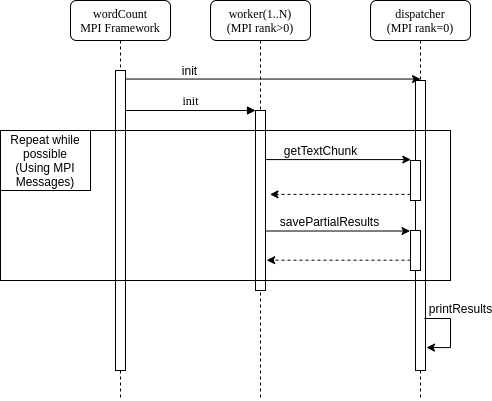
\includegraphics[width=6cm]{wordCountInteraction.png}
		\caption{Entity Interactions}
		\label{wordInteraction}
	\end{figure}
\end{frame}

%----------------------------------------------------------------------------------------
%	 CROSS CORRELATION CALCULATION
%----------------------------------------------------------------------------------------

\section{Cross Correlation Problem}

%------------------------------------------------

\begin{frame}{Multi-Thread Mapping}
	Given that our group had an initial single-thread implementation of the solution for this problem, we needed to map the program to a multi-thread environment and obviously implement it. The necessary mapping were:
	\begin{itemize}
		\item A shared memory space would keep track of the files to be processed.
		\item Each worker would request the shared memory a signal and a specific $\tau$, calculate the cross correlation and return the results to the shared memory.
		\item The shared memory would manage the files content internally enabling the distribution of chunks of text.
		\item The shared memory would keep track of all received results, enabling the program to wite the results no the end of each file or to print to the console the results.
	\end{itemize}
\end{frame}

%------------------------------------------------

\begin{frame}{Solution Diagram}
	\begin{figure}
		\includegraphics[width=5cm]{crossCorrelationDiagram.png}
		\caption{Solution Diagram}
		\label{crossDiagram}
	\end{figure}
\end{frame}

%------------------------------------------------

\begin{frame}{Entity Interaction}
	\begin{figure}
		\includegraphics[width=6cm]{crossCorrelationInteraction.png}
		\caption{Entity Interactions}
		\label{crossInteraction}
	\end{figure}
\end{frame}

\end{document}
